% =============================================================================
%  Rebuilt from the Telegram PDF (proposal.pdf, 19 November 2026 version).
%  Changes requested: team order in "Submitted by" (Monea, Shagato, Snigdha,
%  Kawser, Himel) and Table 3 roles (Kawser = Admin & Tool Lead,
%  Snigdha = Security & Policy Lead).
%  Build:  tectonic proposal_telegram.tex
% =============================================================================
\documentclass[11pt,a4paper]{article}

\usepackage{fontspec}
\defaultfontfeatures{
  Path = /home/sleepycat/.local/share/fonts/onest/,
  Extension = .ttf,
  UprightFont = *-Regular,
  BoldFont = *-Bold,
  ItalicFont = *-Regular,
  ItalicFeatures = {FakeSlant=0.15},
  BoldItalicFont = *-Bold,
  BoldItalicFeatures = {FakeSlant=0.15},
  Scale = 0.92
}
\setmainfont{Onest}
\setsansfont{Onest}
\setmonofont{Onest}

\usepackage[a4paper,top=2.3cm,bottom=2.2cm,left=2.5cm,right=2.5cm]{geometry}
\usepackage{graphicx}
\usepackage{xcolor}
\usepackage{tikz}
\usetikzlibrary{arrows.meta,positioning,calc,shapes.geometric}
\usepackage{array}
\usepackage{tabularx}
\usepackage{colortbl}
\usepackage{caption}
\usepackage{enumitem}
\usepackage[hidelinks]{hyperref}

\newcommand{\projectname}{OS-Buddy}
\definecolor{hdrgrey}{gray}{0.90}
\newcommand{\hdrrow}{\rowcolor{hdrgrey}}
\captionsetup{font=small,labelfont=bf,skip=5pt}
\renewcommand{\arraystretch}{1.15}
\setlength{\parindent}{0pt}
\setlength{\parskip}{0.55em}
\linespread{1.08}

\newcolumntype{P}[1]{>{\raggedright\arraybackslash}p{#1}}
\newcolumntype{Y}{>{\raggedright\arraybackslash}X}
\newcommand{\sect}[1]{\par\vspace{0.5em}{\large\bfseries #1}\par\vspace{0.1em}}

\pagestyle{empty}

\begin{document}
\raggedright

% ============================ COVER PAGE =====================================
\begin{center}
  \vspace*{2.0cm}
  
\includegraphics[width=0.52\textwidth]{../proposal/diu-logo.png}\\[0.9em]
  {\bfseries Faculty of Science and Information Technology}\\
  Department of Computer Science and Engineering\\[2.6em]
  \rule{\linewidth}{0.5pt}\\[2.2em]
  {\fontsize{34}{38}\selectfont\bfseries \projectname}\\[0.6em]
  {\Large An Agentic Operating-System Operator in Bash}\\[2.2em]
  \rule{\linewidth}{0.5pt}\\[1.6em]
  {\small A project proposal submitted for \quad \textbf{CSE324 $|$ Operating Systems Lab}}\\[1.4em]

  {\small\bfseries SUBMITTED BY}\\[0.3em]
  \begingroup\small
  \begin{tabular}{|p{4.7cm}|p{2.0cm}|p{5.5cm}|}
    \hline
    \hdrrow \textbf{Name} & \textbf{Student ID} & \textbf{Email} \\ \hline
    Umma Iman Monea & 241-15-540 & {\footnotesize iman241-15-540@diu.edu.bd} \\ \hline
    Shagato Chowdhury & 241-15-331 & {\footnotesize shagato241-15-331@diu.edu.bd} \\ \hline
    Mst. Washima Zinat Snigdha & 241-15-811 & {\footnotesize zinat241-15-811@diu.edu.bd} \\ \hline
    Md. Kawsar Ahamed & 241-15-309 & {\footnotesize kawsar241-15-309@diu.edu.bd} \\ \hline
    Md Himel Ahmed & 232-15-675 & {\footnotesize ahmed2305101675@diu.edu.bd} \\ \hline
  \end{tabular}\\[1.2em]

  {\small\bfseries SUPERVISED BY}\\[0.3em]
  \begin{tabular}{|p{\dimexpr 12.2cm+4\tabcolsep+2\arrayrulewidth\relax}|}
    \hline
    \hdrrow \textbf{Ms. Tamanna Sultana} \\ \hline
    Lecturer\\
    Department of Computer Science and Engineering\\
    Faculty of Science and Information Technology, Daffodil International University \\ \hline
  \end{tabular}\\[1.2em]
  \endgroup
  {\small 19 November 2026}
\end{center}
\newpage

% ============================ PAGE 2 =========================================
{\LARGE\bfseries Project Proposal}\\[-0.2em]
\rule{\linewidth}{0.5pt}

\sect{Title}
\textbf{OS-Buddy: An Agentic Operating-System Operator in Bash}

\sect{Project Statement}
Our project is based on the following statement from the course project list.

\begingroup\small
\begin{tabularx}{\linewidth}{|Y|}
\hline
\hdrrow \textbf{Assigned project: 9. Shell Script based Project} \\ \hline
Write shell scripts that automate various system administration tasks. These tasks include process management, disk monitoring, backup automation, system health monitoring, and user management. The complexity of the project can vary based on the tasks performed, ranging from simple file handling to more advanced process and network management. \\ \hline
\end{tabularx}
\endgroup

\textbf{What we plan to do:} We will write one shell script for each task in the statement. We will also add one screen that shows everything together. To go further, we will add an AI helper that can do other tasks when the user asks for them in plain English. Every script will show clear results in the terminal and ask before it changes anything (Table~1).

\begin{center}
\captionof{table}{How OS-Buddy will cover the project statement.}
\begingroup\small
\begin{tabularx}{\linewidth}{|P{2.6cm}|P{3.1cm}|Y|}
\hline
\hdrrow \textbf{Task in the statement} & \textbf{Planned command} & \textbf{What it will do} \\ \hline
Process management & os-buddy proc & Show running programs, find one by name, and stop it after asking. \\ \hline
Disk monitoring & os-buddy disk & Show how full each disk is and warn when it is almost full. \\ \hline
Backup automation & os-buddy backup & Save important folders as backup files, check them, restore them, and run backups on a schedule. \\ \hline
System health monitoring & os-buddy health, os-buddy status & Show the CPU, memory, disk and uptime in one easy report with a simple verdict. \\ \hline
User management & os-buddy users & List, add, lock and remove user accounts, while protecting important accounts. \\ \hline
Simple files up to advanced process and network management & AI helper: os-buddy “goal” & Do other tasks written in plain English, such as finding files or checking running programs, following safety rules. \\ \hline
\end{tabularx}
\endgroup
\end{center}

\sect{Description}
Using a Unix system means remembering many commands and knowing which ones are risky. \textbf{OS-Buddy} will make this easier. The user will describe a goal in plain English, such as “find the biggest files in this folder”. The AI helper will choose the steps, carry them out, check the results, and keep going until the goal is done, or say clearly that it could not do it. It will be written in Bash and will use Google’s Gemini AI to choose each step.

\textbf{A safety layer will sit between the AI and the computer:} Safe commands that only read information will run on their own, anything that changes something will ask the user first, and dangerous commands will always be blocked. OS-Buddy will work on Linux and similar systems, either as a chat or as a single command for one task. The admin scripts in Table~1 will work without any AI.
\newpage

% ============================ PAGE 3 =========================================
\sect{Problem and Objectives}
AI tools can suggest shell commands, but running them without checking can be unsafe, and most chat tools leave the checking to the user. This project will build a helper that completes tasks while keeping the user in control. Our objectives are:
\begin{itemize}[itemsep=0pt,topsep=2pt,parsep=0pt,leftmargin=2em]
  \item an AI helper that plans a task, does it and checks the result;
  \item safety rules that decide what runs freely, what needs approval and what is blocked;
  \item simple admin scripts for the five tasks, which work without AI;
  \item a reliable connection to the Gemini AI that keeps the secret key safe;
  \item tests that show everything works on Mac and Linux.
\end{itemize}

\sect{Design Approach and Scope}
We will describe the helper with the PEAS model (Table~2), which lists what the helper aims for, where it works, what it can do and what it can sense. The code will be split into small parts that each do one job, so it is easy to read and change. \emph{Out of scope:} running directly on Windows, a graphical interface, and any change made without the user’s approval.

\begin{center}
\captionof{table}{PEAS summary of OS-Buddy.}
\begingroup\small
\begin{tabularx}{\linewidth}{|>{\bfseries}P{2.2cm}|Y|}
\hline
\hdrrow Component & \textbf{Specification} \\ \hline
Performance & Finish the task correctly, follow the safety rules, recover from mistakes, and stop after a reasonable number of steps. \\ \hline
Environment & A Linux or Unix computer, a person at the terminal, and the Gemini AI service. \\ \hline
Actuators & Run commands, read and write files, ask the user questions, and run the admin scripts, always through the safety rules. \\ \hline
Sensors & What commands print, file contents, facts about the computer, and the user’s replies. \\ \hline
\end{tabularx}
\endgroup
\end{center}

\sect{How the Agent Works}
Figure~1 shows who uses OS-Buddy and what they can do. The user gives a goal, approves or denies changes, and answers questions. The Gemini AI only plans; the computer is only touched through the safety rules. The admin scripts need neither the AI nor a network.

Figure~2 follows one goal from the first word the user types to the final answer. The helper repeats a short loop. It asks Gemini what to do next, checks the chosen action with the safety rules, runs it only if allowed, and sends the result back to Gemini. The loop ends when Gemini answers without asking for another action, which is how the goal is reached. If an action is blocked or denied, Gemini is told and must choose another way. The loop also stops with a clear message after 30 steps.
\newpage

% ============================ FIGURE 1 =======================================
\thispagestyle{empty}
\vspace*{\fill}
\begin{center}
\begin{tikzpicture}[
  >=Stealth, font=\scriptsize,
  uc/.style={ellipse, draw, fill=white, align=center, inner sep=2pt, minimum height=0.85cm, minimum width=4.0cm},
  lab/.style={font=\tiny\itshape, fill=white, inner sep=1pt}
]
  % stick figure
  \newcommand{\actor}[3]{% x, y, label
    \draw (#1,#2+0.45) circle (0.13);
    \draw (#1,#2+0.32) -- (#1,#2-0.08);
    \draw (#1-0.22,#2+0.2) -- (#1+0.22,#2+0.2);
    \draw (#1,#2-0.08) -- (#1-0.18,#2-0.40);
    \draw (#1,#2-0.08) -- (#1+0.18,#2-0.40);
    \node[align=center, anchor=north] at (#1,#2-0.45) {#3};}

  \draw (0,0) rectangle (11.3,8.3);
  \node[anchor=north west, font=\small\bfseries] at (0.15,8.2) {OS-Buddy system};

  \node[uc] (chat)  at (3.0,7.2) {Chat with memory};
  \node[uc] (goal)  at (3.0,5.5) {\textbf{Give a goal in plain English}\\[-1pt]{\tiny (AI helper)}};
  \node[uc] (ques)  at (3.0,3.8) {Answer a question\\[-1pt]{\tiny from the helper}};
  \node[uc] (appr)  at (3.0,2.5) {Approve or deny a change};
  \node[uc, minimum width=4.6cm] (admin) at (3.4,1.0) {Run an admin task\\[-1pt]{\tiny proc, disk, backup, health, users}};

  \node[uc, minimum width=3.6cm] (plan) at (8.6,7.0) {Plan the next step};
  \node[uc, minimum width=3.6cm] (run)  at (8.6,5.4) {Run a command, read or\\edit a file};
  \node[uc, minimum width=3.6cm] (chk)  at (8.6,3.6) {Check the safety rules};

  \actor{-1.5}{4.5}{User}
  \actor{-1.0}{1.1}{Scheduler\\(cron)}
  \actor{12.9}{7.0}{Gemini AI\\(external)}
  \actor{12.9}{3.6}{Operating\\system}

  % associations
  \draw (-1.35,4.6) -- (chat.west);
  \draw (-1.35,4.5) -- (goal.west);
  \draw (-1.35,4.4) -- (ques.west);
  \draw (-1.35,4.3) -- (appr.west);
  \draw (-1.35,4.2) -- (admin.west);
  \draw (-0.85,1.1) -- (admin.west);
  \draw (plan.east) -- (12.75,7.0);
  \draw (run.east) -- (12.75,3.7);
  \draw (admin.east) -- (12.75,3.5);

  % include / extend
  \draw[dashed,->] (goal.north) -- node[lab,right,xshift=2pt] {\guillemotleft include\guillemotright} (chat.south);
  \draw[dashed,->] (ques.north) -- node[lab,right,xshift=2pt] {\guillemotleft extend\guillemotright} (goal.south);
  \draw[dashed,->] (goal.north east) -- node[lab,above] {\guillemotleft include\guillemotright} (plan.west);
  \draw[dashed,->] (goal.east) -- node[lab,above] {\guillemotleft include\guillemotright} (run.west);
  \draw[dashed,->] (goal.south east) -- node[lab,above,pos=0.35] {\guillemotleft include\guillemotright} (chk.north west);
  \draw[dashed,->] (appr.east) -- node[lab,above] {\guillemotleft extend\guillemotright} (chk.south west);
\end{tikzpicture}

\captionof{figure}{Use case diagram of OS-Buddy. Dashed arrows are \emph{include} (always done) and \emph{extend} (only when needed, for example approval is asked only when the safety rules say “ask”).}
\end{center}
\vspace*{\fill}
\newpage

% ============================ FIGURE 2 =======================================
\thispagestyle{empty}
\begin{center}
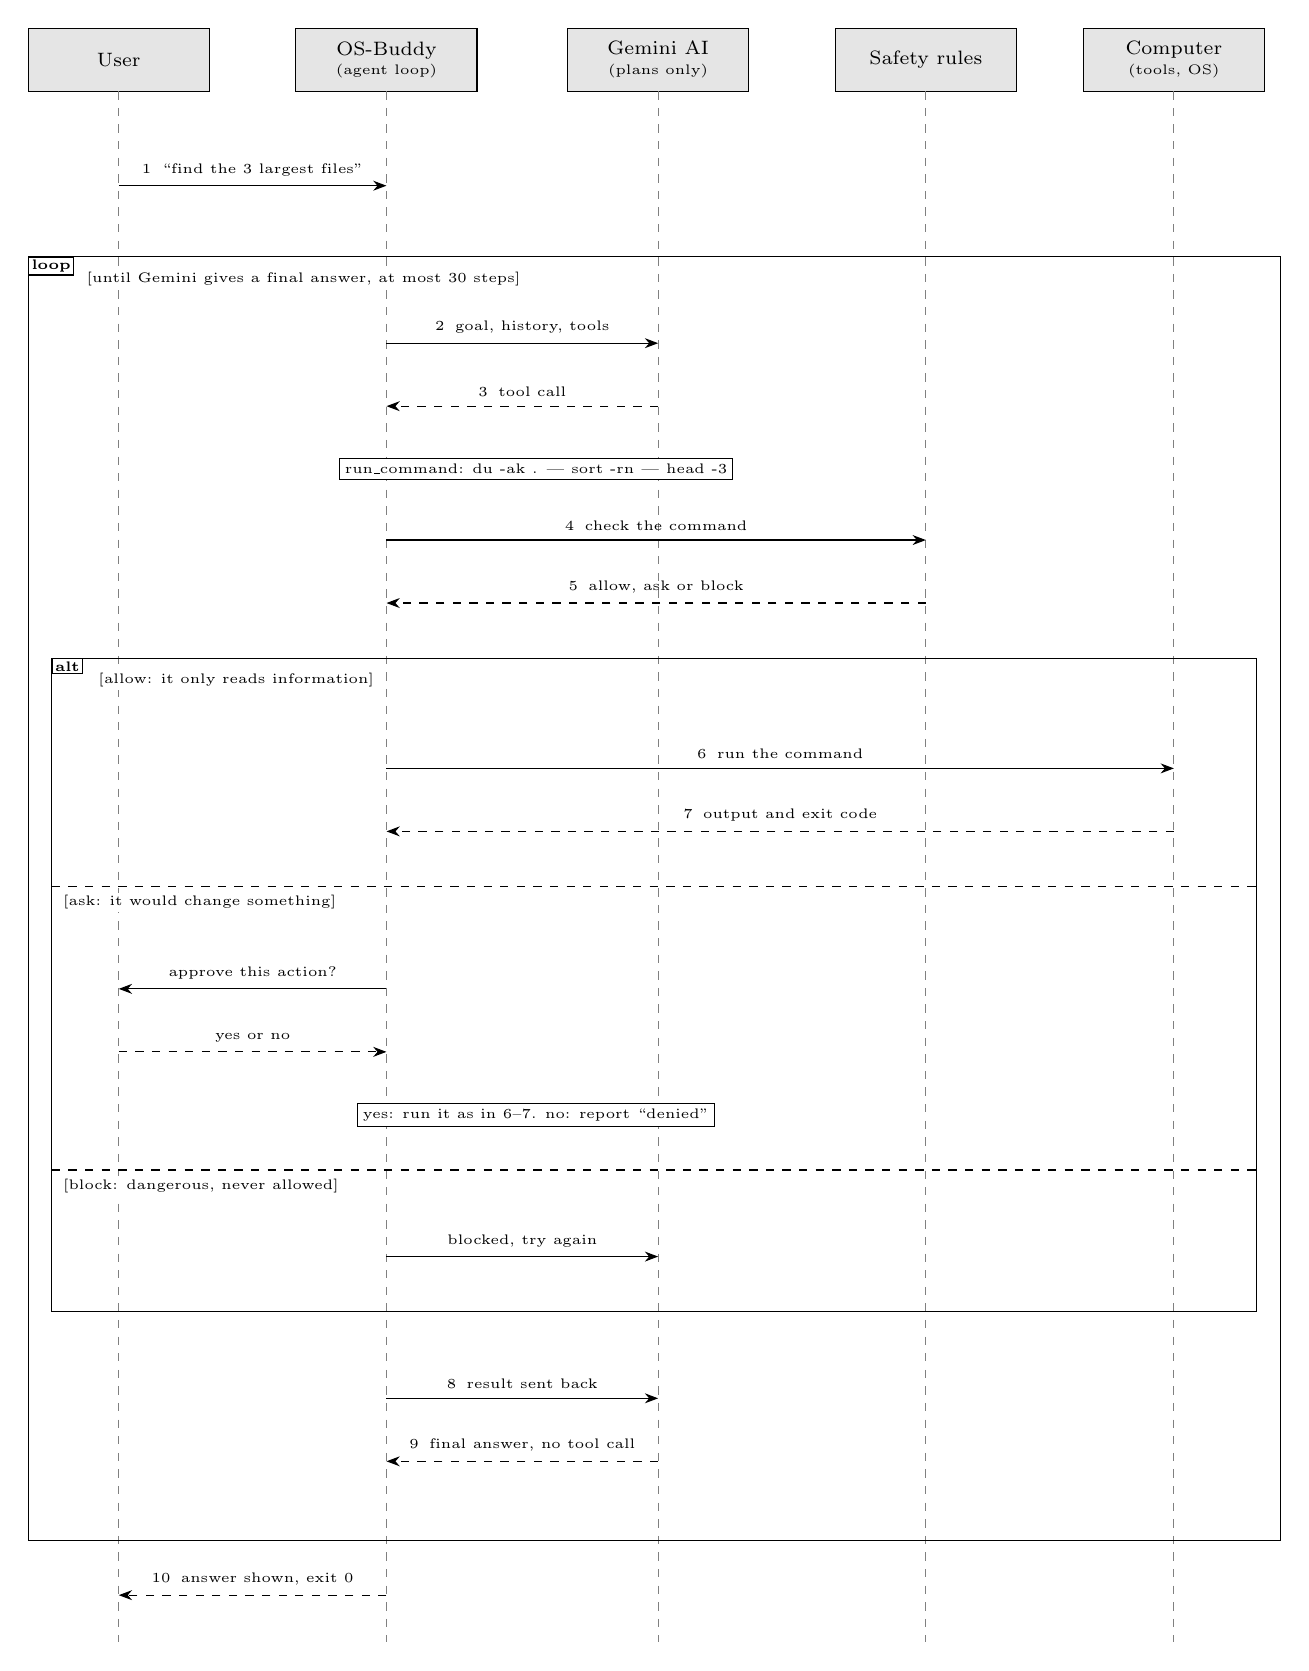
\begin{tikzpicture}[
  >=Stealth, font=\scriptsize,
  hd/.style={draw, fill=hdrgrey, align=center, minimum width=2.3cm, minimum height=0.8cm, inner sep=2pt},
  life/.style={dashed, gray},
  note/.style={draw, fill=white, inner sep=2pt, font=\tiny},
  guard/.style={anchor=west, font=\tiny, fill=white, inner sep=1pt}
]
  % x positions
  \def\xU{0}\def\xO{3.4}\def\xG{6.85}\def\xS{10.25}\def\xC{13.4}
  \node[hd] at (\xU,0) {User};
  \node[hd] at (\xO,0) {OS-Buddy\\[-1pt]{\tiny (agent loop)}};
  \node[hd] at (\xG,0) {Gemini AI\\[-1pt]{\tiny (plans only)}};
  \node[hd] at (\xS,0) {Safety rules};
  \node[hd] at (\xC,0) {Computer\\[-1pt]{\tiny (tools, OS)}};
  \foreach \x in {\xU,\xO,\xG,\xS,\xC} \draw[life] (\x,-0.4) -- (\x,-20.1);

  % message macros: #1 y, #2 from, #3 to, #4 text
  \newcommand{\msg}[4]{\draw[->] (#2,#1) -- node[above,pos=0.5,font=\tiny] {#4} (#3,#1);}
  \newcommand{\ret}[4]{\draw[->,dashed] (#2,#1) -- node[above,pos=0.5,font=\tiny] {#4} (#3,#1);}

  \msg{-1.6}{\xU}{\xO}{1\;\;“find the 3 largest files”}

  % loop frame
  \draw (-1.15,-2.5) rectangle (14.75,-18.8);
  \node[draw,fill=white,anchor=north west,inner sep=1pt,font=\tiny\bfseries] at (-1.15,-2.5) {loop};
  \node[guard] at (-0.45,-2.78) {[until Gemini gives a final answer, at most 30 steps]};

  \msg{-3.6}{\xO}{\xG}{2\;\;goal, history, tools}
  \ret{-4.4}{\xG}{\xO}{3\;\;tool call}
  \node[note] at (\xO+1.9,-5.2) {run\_command: du -ak . | sort -rn | head -3};
  \msg{-6.1}{\xO}{\xS}{4\;\;check the command}
  \ret{-6.9}{\xS}{\xO}{5\;\;allow, ask or block}

  % alt frame
  \draw (-0.85,-7.6) rectangle (14.45,-15.9);
  \node[draw,fill=white,anchor=north west,inner sep=1pt,font=\tiny\bfseries] at (-0.85,-7.6) {alt};
  \node[guard] at (-0.3,-7.88) {[allow: it only reads information]};
  \msg{-9.0}{\xO}{\xC}{6\;\;run the command}
  \ret{-9.8}{\xC}{\xO}{7\;\;output and exit code}
  \draw[dashed] (-0.85,-10.5) -- (14.45,-10.5);
  \node[guard] at (-0.75,-10.7) {[ask: it would change something]};
  \msg{-11.8}{\xO}{\xU}{approve this action?}
  \ret{-12.6}{\xU}{\xO}{yes or no}
  \node[note] at (\xO+1.9,-13.4) {yes: run it as in 6--7. no: report “denied”};
  \draw[dashed] (-0.85,-14.1) -- (14.45,-14.1);
  \node[guard] at (-0.75,-14.3) {[block: dangerous, never allowed]};
  \msg{-15.2}{\xO}{\xG}{blocked, try again}

  \msg{-17.0}{\xO}{\xG}{8\;\;result sent back}
  \ret{-17.8}{\xG}{\xO}{9\;\;final answer, no tool call}

  \ret{-19.5}{\xO}{\xU}{10\;\;answer shown, exit 0}
\end{tikzpicture}

\captionof{figure}{Sequence diagram of one goal. Gemini only chooses actions; every action passes the safety rules before it reaches the computer, and each result goes back to Gemini until the goal is reached.}
\end{center}
\newpage

% ============================ PAGE 6 =========================================
\sect{Team Contributions}
The project will be done by a group of five. Each member will take one main area, so everyone can work at the same time.

\begin{center}
\captionof{table}{Division of work within the group.}
\begingroup\small
\begin{tabularx}{\linewidth}{|P{3.2cm}|P{3.4cm}|Y|}
\hline
\hdrrow \textbf{Member} & \textbf{Main area} & \textbf{What they will do} \\ \hline
Umma Iman Monea & Overall design and AI helper & Plan the design, build the main AI helper and the start of the program \\ \hline
Md. Kawsar Ahamed & Admin and tool lead & Build the actions the helper can take and the admin scripts \\ \hline
Shagato Chowdhury & Gemini connection & Connect to the Gemini AI and write its instructions \\ \hline
Mst. Washima Zinat Snigdha & Security and policy lead & Write the safety rules and the approval questions \\ \hline
Md Himel Ahmed & Testing and documents & Write the tests, set up automatic checks, and prepare the project documents \\ \hline
\multicolumn{3}{|l|}{\cellcolor{hdrgrey}\textbf{Shared by the whole group}} \\ \hline
\multicolumn{3}{|l|}{Planning, design decisions, checking each other’s work, demonstration} \\ \hline
\end{tabularx}
\endgroup
\end{center}

\sect{References}
\begingroup\small
\begin{enumerate}[itemsep=0pt,topsep=2pt,parsep=0pt,leftmargin=2em]
  \item S. Russell and P. Norvig, \emph{Artificial Intelligence: A Modern Approach}, 4th ed., Pearson, 2020.
  \item Google AI for Developers, “Gemini API documentation: Function calling,” https://ai.google.dev/gemini-api/docs/function-calling.
  \item GNU Project, \emph{Bash Reference Manual}, https://www.gnu.org/software/bash/manual/.
\end{enumerate}
\endgroup

\end{document}
